\section{Feynman Diagrams}
\subsection{Feynman Rules}
Last time, we did a perturbative calculation of something. We did it with a straightforward Taylor expansion (in the coupling constant) of the functional integral expression for the two-point function, and then used our ability to do Gaussian functional integrals to get the result. But we never actually did a functional integral! We already did that previously (Wick's Theorem) so we just quoted the result of that - the only thing left to do was to do the combinatorics of the interactions. In doing so, we were able to work out these combinatorics in a straightforwards way using Feynman diagrams. As you imagine, all of this can be automated somehow (and in fact there are packages that draw all Feynman diagram that contribute to some order to some correlation functions), and this is a usually nice thing to use. It's easy to forget if you do it by hand... (anecdote about a group who worked on Yang-Mills for many years, but had forgotten just one diagram, and got scooped by a group in Russia). There's quite a bit to the science of Feynman diagrams, and in this course we just scratch the surface. We already used them last time, and now let's use them some more. One thing we might have noticed from last time is there are rules for how to begin and how to do the computation. These we can formalize and turn into a list of \emph{Feynman Rules} - we don't copy them here, but look in the textbook for a full list! For simple computations, you will find that it is straightforwards, but the computation quickly begins to increase at higher order in perturbation theory.

\subsection{Simplification 1 - Momentum Space}
Recall our (first-order) perturbative computation of the two-point function:
\begin{equation}\label{eq-Dxy}
    D(x, y) = \Delta(x, y) - \frac{i\lambda}{2}\int dz \Delta(x, y)\Delta(z, z)\Delta(z, y) - i\lambda \int dz \Delta(x, z)(-z^{(1)}\p^2 + z^{(1)}_m m^2)\Delta(z, y) + \ldots
\end{equation}
Now using that $D(x, y) = D(x - y)$ and so $\Delta(x, y) = \Delta(x - y)$ (from our Lorentz invariant symmetry analysis of two-point correlation functions from earlier), we find that the above expression turns into convolutions. This expression therefore simplifies drastically (into just a product) if we take a Fourier transform and look at momentum space. We therefore can simplify by going into momentum space:
\begin{equation}
    D(x, y) = \int \frac{d^4k}{(2\pi)^4}e^{ik^\mu(x - y)_\mu}D(k^2)
\end{equation}
for the free-field propogator, we know exactly what it is:
\begin{equation}
    \Delta(x, y) = \int \frac{d^4k}{(2\pi)^4}e^{ik^\mu (x - y)_\mu} \frac{-i}{k^2 + m^2 - i\e}
\end{equation}
So if we substitute this into \eqref{eq-Dxy}, we find:
\begin{equation}
    \begin{split}
        D(k^2) &= \frac{-i}{k^2 + m^2 - i\e} + \frac{-i}{k^2 + m^2 - i\e}\left(-\frac{i\lambda}{2}\int \frac{d^4p}{(2\pi)^4}\frac{-i}{p^2 + m^2 - i\e}\right)
        \frac{-i}{k^2 + m^2 - i\e} 
        \\ &+ \frac{-i}{k^2 + m^2 - i\e}\left(-i\lambda(z^{(1)}k^2 + z^{(1)}_m m^2)\right)\frac{-i}{k^2 + m^2 - i\e} + \ldots
    \end{split}
\end{equation}
so to get a closed form expression, the only thing we have to do is calculate the integral appearing in the above expression. Unfortunately, the integral is divergent. However, if we just integrate over $p^0$ its convergent, and we have the same integral as we looked at a couple lectures ago (where we calculated a first-order energy shift, and then could absorb this shift into the mass, which was formally infinite...). It is a very similar story to what we had before, but more systematic. One such way this is so is that the integral is Lorentz covariant.

One last thing is the counterterms sitting there; we can choose $z_m^{(1)}$ to cancel the integral and $z^{(1)} = 0$ as there is no other $k^2$ dependence. This would be an ok thing to do, but there is an arbitrariness in choosing the counterterms, known as scheme dependence. If the integral had $k$ dependence, we would have to be more carful...

The second thing to notice is the form of this expression. Drawing them diagramatically, we have:

\begin{center}
    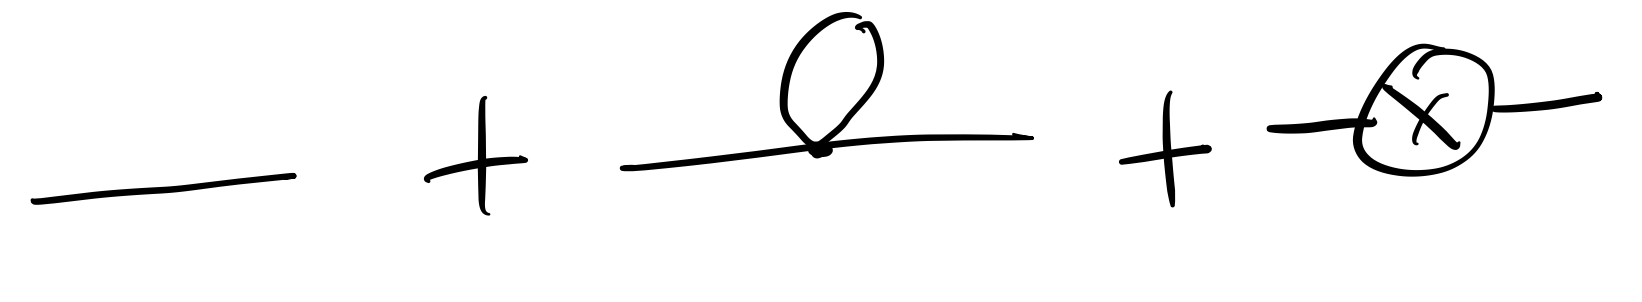
\includegraphics[scale=0.3]{Images/fig-lec27feynman1.png}
\end{center}

If we continued to higher orders, we first have repetitions of what came before (but now in pairs):

\begin{center}
    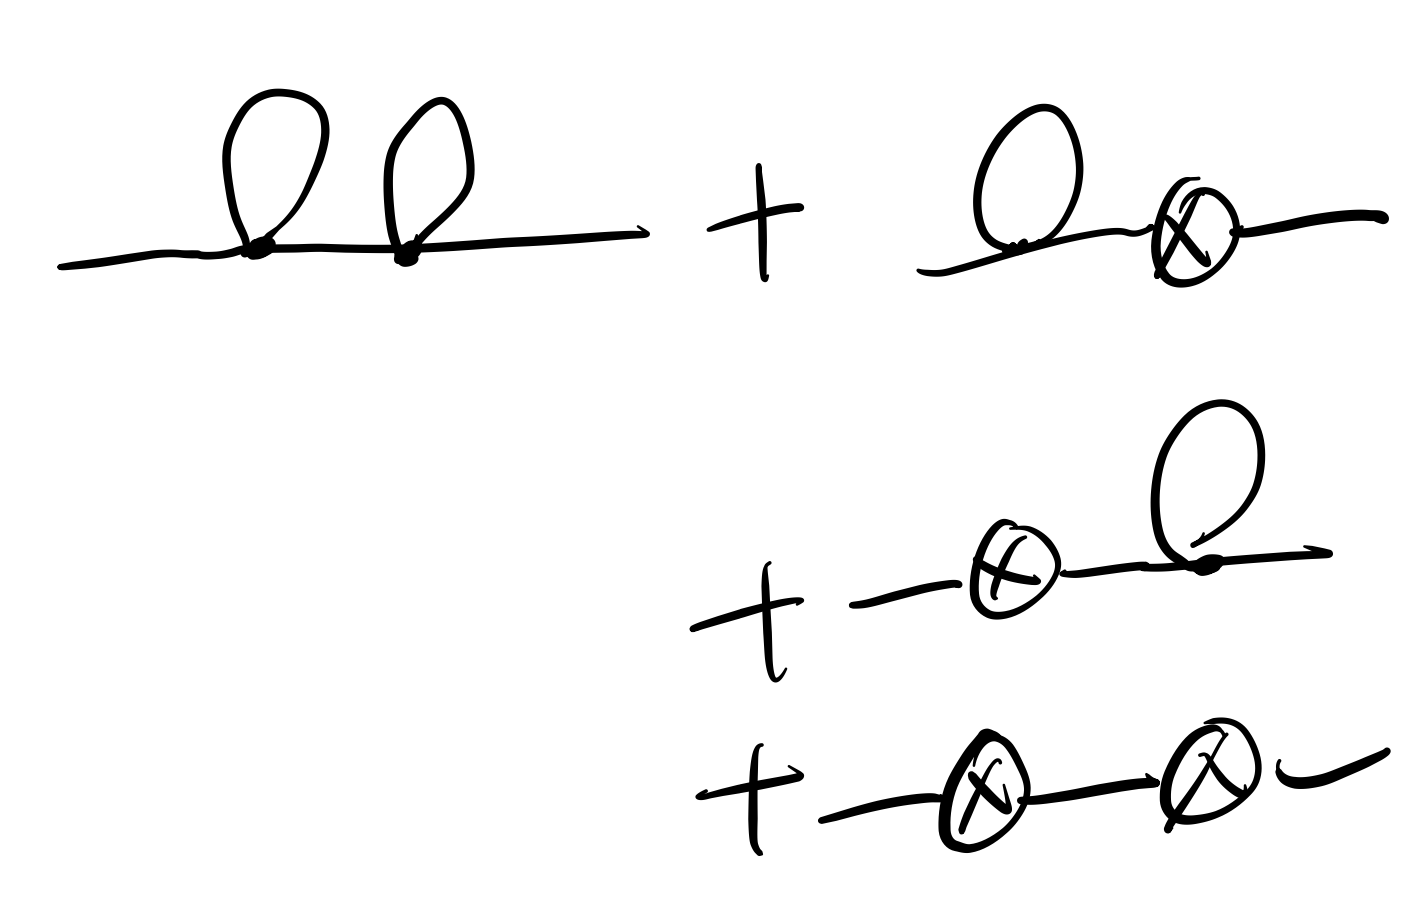
\includegraphics[scale=0.3]{Images/fig-lec27feynman2.png}
\end{center}

But also new terms:

\begin{center}
    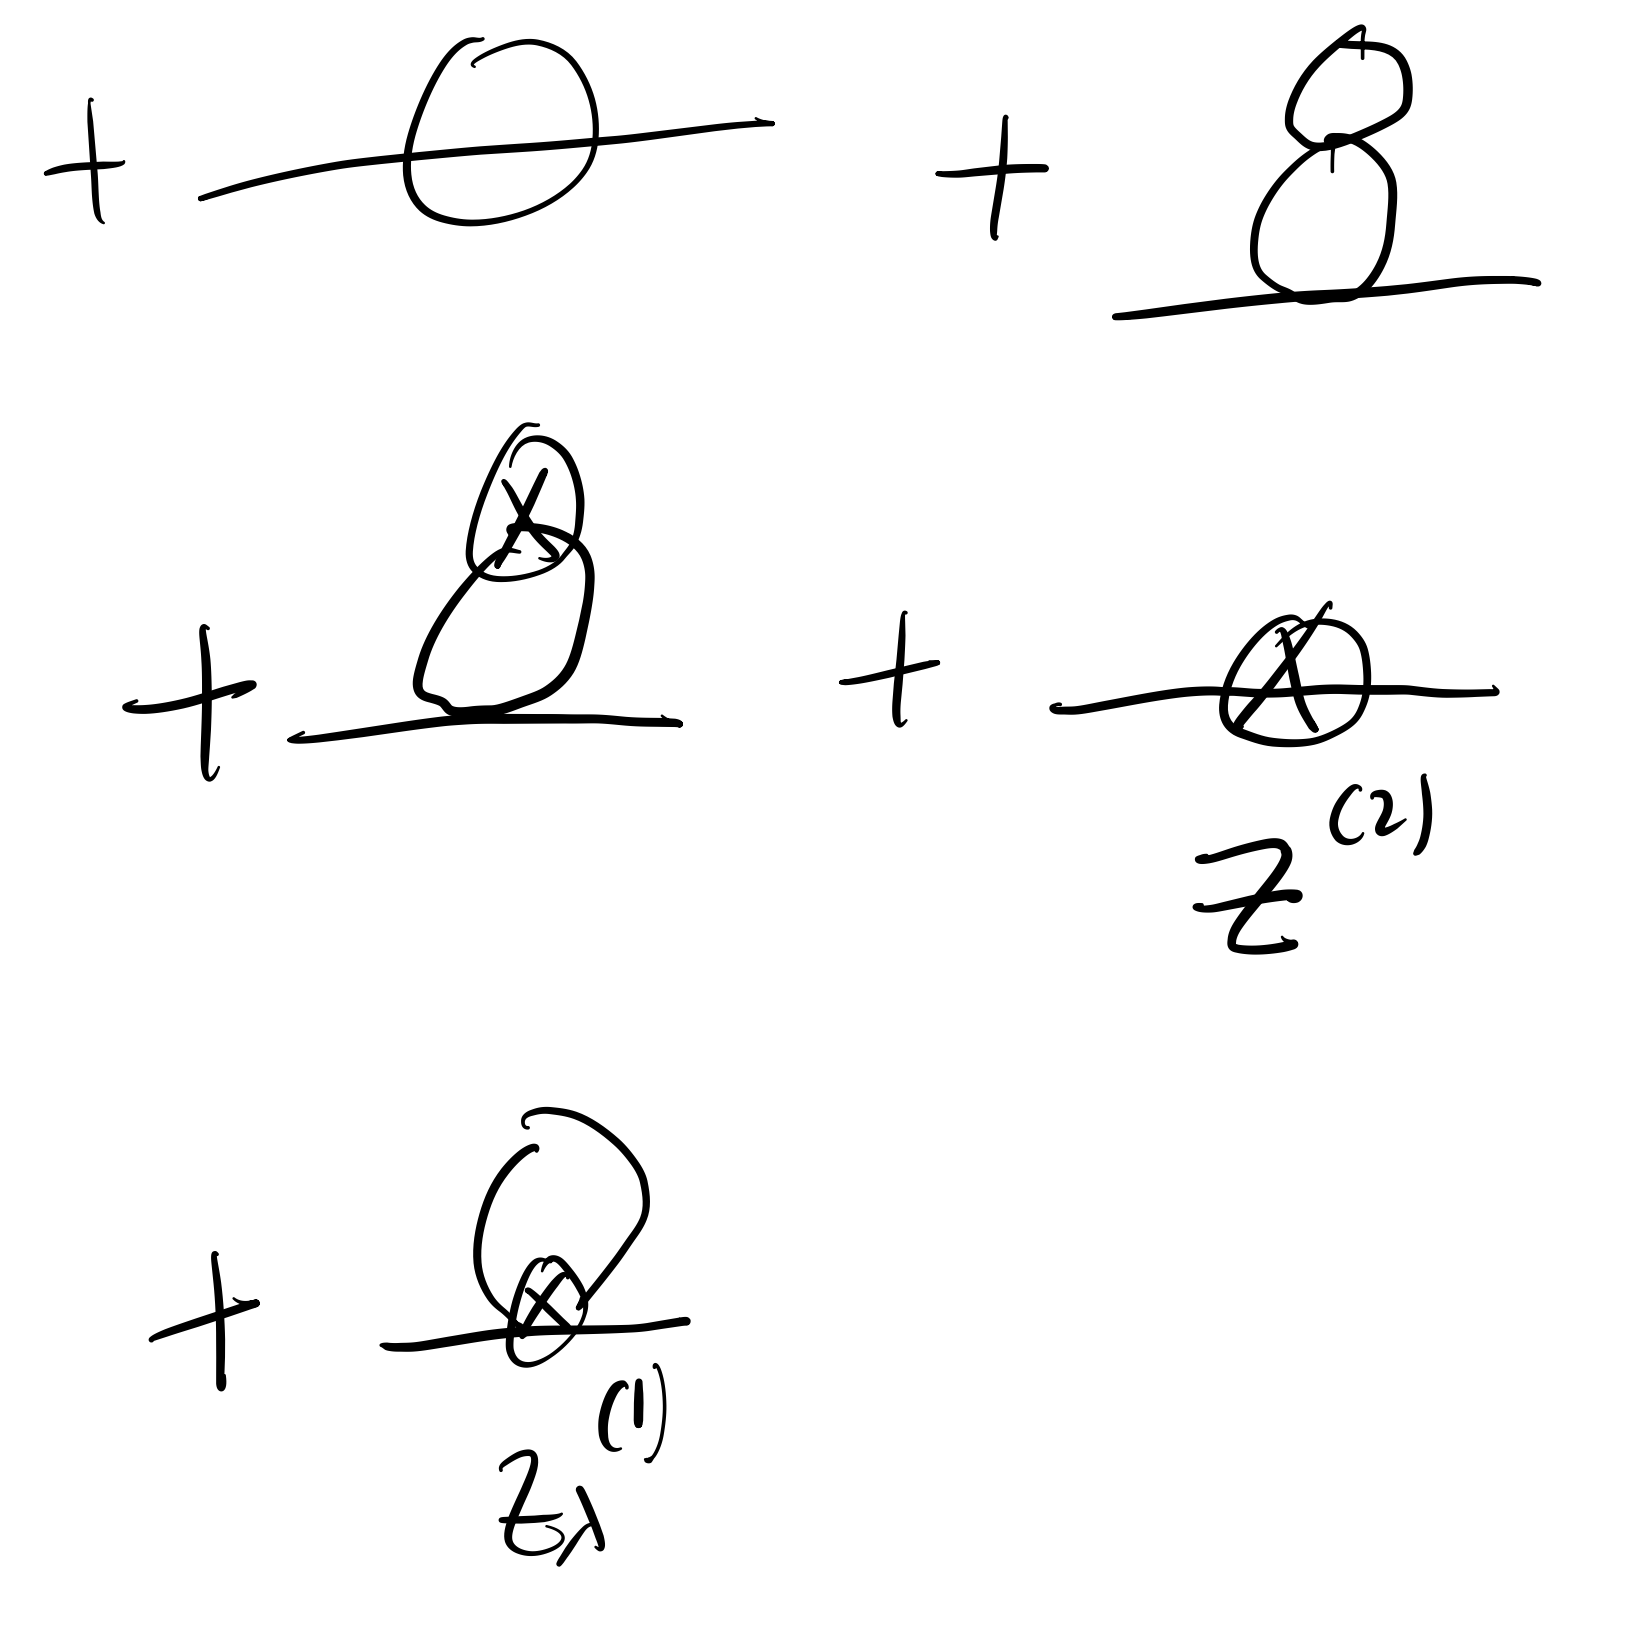
\includegraphics[scale=0.3]{Images/fig-lec27feynman3.png}
\end{center}

Which is all the terms to order $\lambda^2$ - this already seems like a lot! Is there any way to systematically simplify or distinguish? Yes, you can topologically characterize the diagrams . It would be useful if it allowed us to forget about some terms. In fact we can. We can categorize reducible and irreducible diagrams. Irreducible - can't snip somewhere and retain something non-trivial. So, the reducible ones are the repeated (paired) diagrams here, and the irreducible ones are the new ones. The question is then; is it possible to just focus on the irreducible diagrams and obtain all diagrams from there?

\subsection{Simplification 2 - Compute Connected, Irreducible Diagrams}
Yes. We consider an expansion as follows:

\begin{center}
    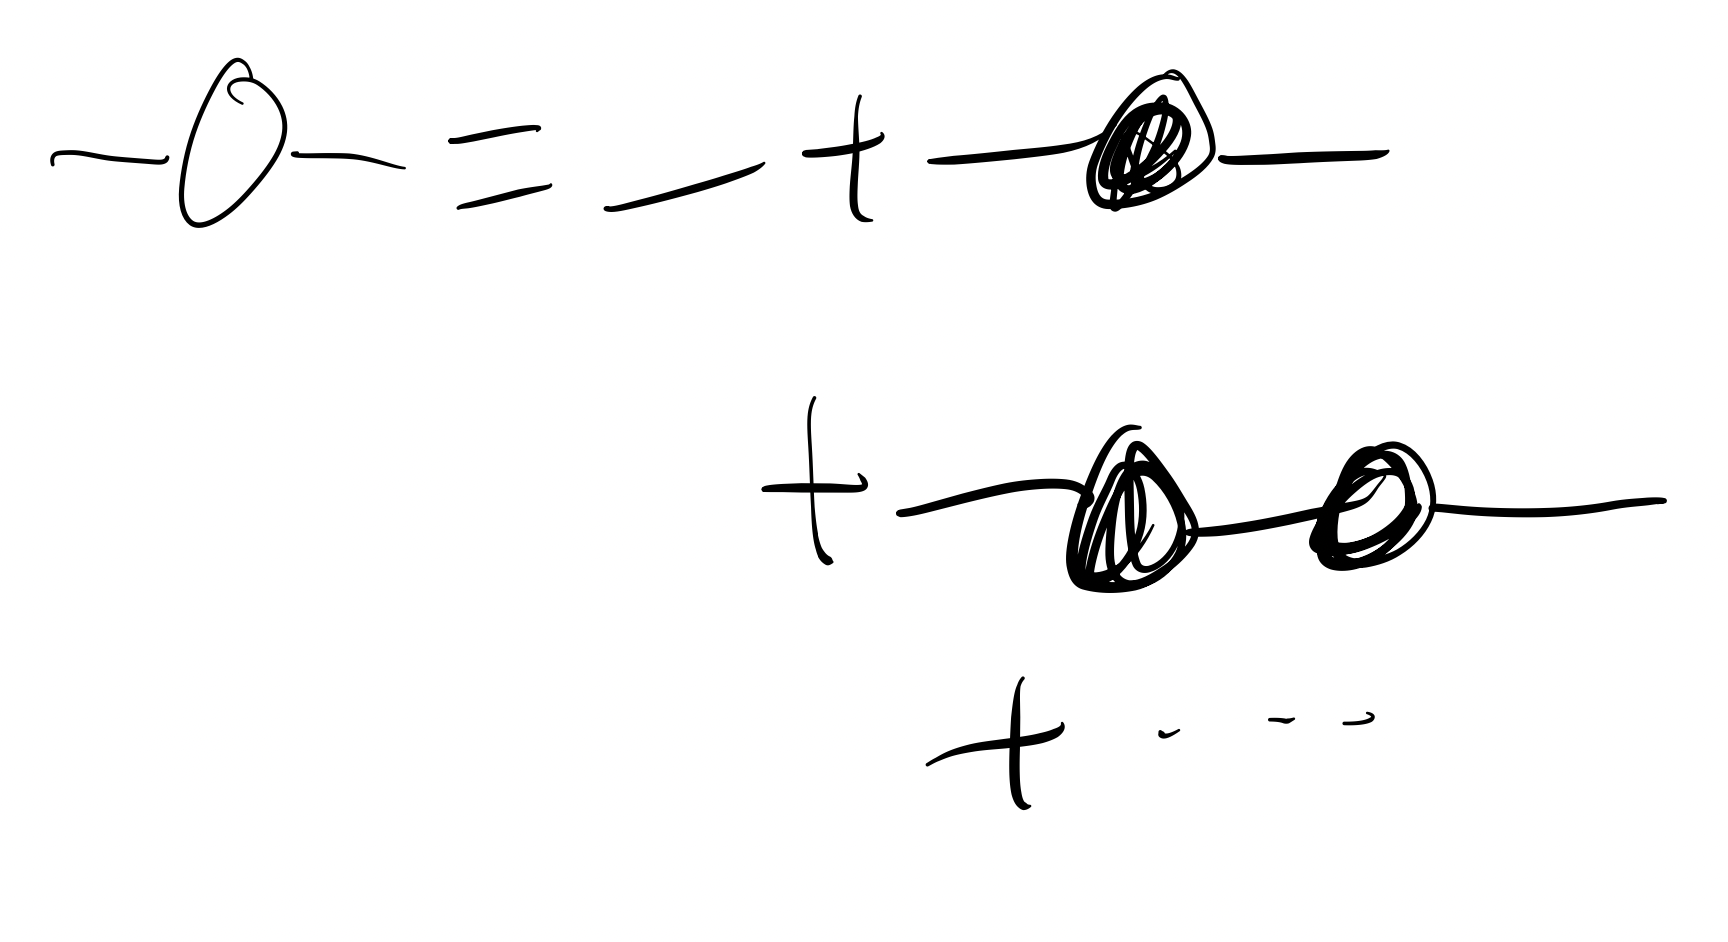
\includegraphics[scale=0.3]{Images/fig-lec27feynman4.png}
\end{center}

Where the black dots correspond to irreducible diagrams. Ones that are repetitions of what we have already calculated are obtained by joining irreducible (sometimes called one-particle irreducible) diagrams together. This cuts down on the multiplicity significantly. Note that when we put things together, the combinatorial factors organize themselves such that this is just a simple geometric series. Gordon doesn't know an easy way to prove this; every QFT textbook simply states it. The textbook gives a proof sketch, but it is complicated.

Consider the computation of a four-point function. Some diagrams that contribute here are disconnected two-point diagrams. These contribute a lot of multiplicity and it would be nice to only have to focus on the connected ones. However, we need a well-defined way to put them back together to get the full result. It turns out there is a rather clever way. We've chosen a field theory with a symmetry such that every diagram needs two legs coming out of it.

\begin{center}
    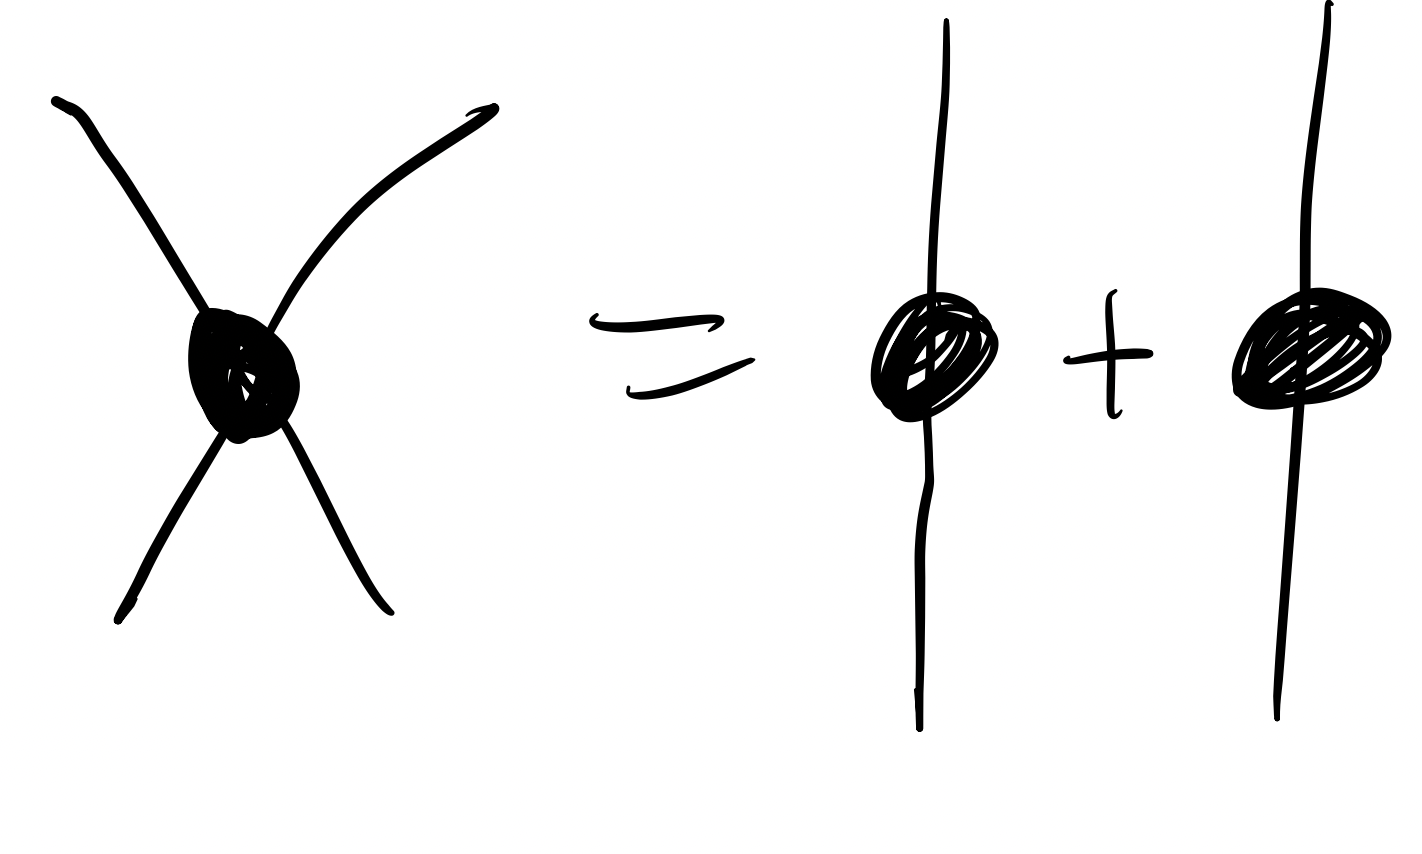
\includegraphics[scale=0.3]{Images/fig-lec27feynman5.png}
\end{center}

We already knew it before this discussion, but also note a \textbf{Simplification 0} of sorts - \textbf{Goldstone's Theorem}!

\subsection{Diagram Combinatorics - Connected Correlation Functions}
We wouldn't be able to discuss this meaningfully without knowing the combinatorics involved. In fact there are functional methods involved here. Let us discuss the case of connected correlation functions. Given the generating functional $Z[J]$, we then have $W[J] = \ln Z[J]$ is the generating functional for connected correlation functions. So in other words, the connected correlation function is:
\begin{equation}
    \Gamma_C(x_1, \ldots x_n) = \left.\frac{1}{i}\frac{\delta}{\delta J(x_1)} \ldots \frac{1}{i}\frac{\delta}{\delta J(x_n)}W[J]\right|_{J = 0}
\end{equation}
We thus obtain a formula for connected correlation functions in terms of ordinary ones. For two-point correlation functions this formula is almost trivial:
\begin{equation}
    \Gamma_C(x_1, x_2) = D(x_1, x_2) - \avg{\varphi(x_1)}\avg{\varphi(x_2)}
\end{equation}
but in the field theory we work with I believe the expectation values vanish. For the four-point function, we get something a little more complicated:
\begin{equation}
    \Gamma_C(x_1, x_2, x_3, x_4) = \Gamma(x_1, x_2, x_3, x_4) - \Gamma(x_1, x_2)\Gamma(x_3, x_4) - \Gamma(X_1, x_3)\Gamma(x_2, x_4) - \Gamma(x_1, x_4)\Gamma(x_2, x_3)
\end{equation}
where $\Gamma$ without the $C$ denotes the time ordered $n$-point correlation function. We may want to invert this, as we want the time-ordered correlation functions in terms of the connected ones, rather than the other way around. 

Note - see the proof in the textbook for more details - we see that the expansion of a connected correlators in Feynman diagrams only use connected Feynman diagrams. We can do the same thing for the irreducible correlation functions (connected connected and irreducible correlation functions). This is a bit interesting, though we will not have a lot of time for it here. It will involve the Legendre transform, and it will come up often in a statistical mechanics class.

\subsection{Generating Functional for Irreducible Correlation Functions}
We will just talk about correlation functions for a moment, not Feynman diagrams. We will then define what we mean by irreducible in this context, and then it can be shown that such correlation functions can be written as a sum of irreducible Feynman diagrams. What we do is we return to $W[J]$, the connected generating functional. Let us define the one-point function as:
\begin{equation}
    \phi(x) = \frac{1}{i}\frac{\delta}{\delta J(x)}W[J]
\end{equation}
which differs a lot from the connected one-point function as we do not set $J = 0$. Then, take $W$ and do a Legendre transform:
\begin{equation}
    \Gamma[\phi] = W[J] - i\int J(x)\phi(x)
\end{equation}
What we must do is take the equation for $\phi$ and solve it for $J$ - this is terrible, so we solve it perturbatively. We then plug it in to get $\Gamma$ as a functional of $\phi$. And then, using the same terrible notation, the irreducible $n$-point function is obtained via functional derivatives of the classical field:
\begin{equation}
    \Gamma_I(x_1, \ldots x_n) = \left.\frac{1}{i}\frac{\delta}{\delta \phi(x_1)} \ldots \frac{1}{i}\frac{\delta}{\delta \phi(x_n)}\Gamma[\phi]\right|_{\phi = ?}
\end{equation}
and then we set $J = 0$, which seems hard as we've lost track of $J$. We can see that taking the functional derivative of $\Gamma[\phi]$:
\begin{equation}
    \frac{1}{i}\frac{\delta \Gamma[\phi]}{\delta \phi(x)} = -J(x)
\end{equation}
so to put $J = 0$, we find a $\phi$ which is a soloution to the above equation, so $\Gamma$ is at an extremum as a functional of $\phi$:
\begin{equation}
    \Gamma_I(x_1, \ldots x_n) = \left.\frac{1}{i}\frac{\delta}{\delta \phi(x_1)} \ldots \frac{1}{i}\frac{\delta}{\delta \phi(x_n)}\Gamma[\phi]\right|_{\phi = \bar{\phi}}
\end{equation}
where:
\begin{equation}
   \left. \frac{1}{i}\frac{\delta \Gamma}{\delta \phi}\right|_{\phi = \bar{\phi}} = 0.
\end{equation}
Usually $\bar{\phi} = 0$, but it doesn't have to be, e.g. when we have spontaneous symmetry breaking, where we have multiple zeroes and have to choose based on stability criteria, e.g. taking the second derivative and seeing if one has a sensible two-point function. We won't worry too much about this. What we really need is just a systematic realtionship between $\Gamma_I$ and the $\Gamma$ connected, $\Gamma$ unindexed... for example:
\begin{equation}
    \left.\frac{1}{i^2}\frac{\delta^2\Gamma}{\delta\phi(x_1)\delta\phi(x_2)}\right|_{\phi = \bar{\phi}} = D^{-1}(x, y)
\end{equation}
and then we can calculate higher ones, and the relationship between them and the ordinary correlation functions is one that removes all the pieces. Then, one can actually prove that the sum of irreducible diagrams produces an irreducible correlation functions.

This is a long story, and probably at the edge/beyond the edge of the curriculum of the course. The moral is that we can calculate irreducible diagrams, and then somewhere dig up an algorithm for reconstructing the full $n$-point function by these mechanism. Almost nobody does this in detail because you learn it via looking at a few simple correlation functions (e.g. two point is very simple). But its good to know something systematic is out there.